% Created by tikzDevice version 0.12.3.1 on 2021-12-16 22:51:20
% !TEX encoding = UTF-8 Unicode
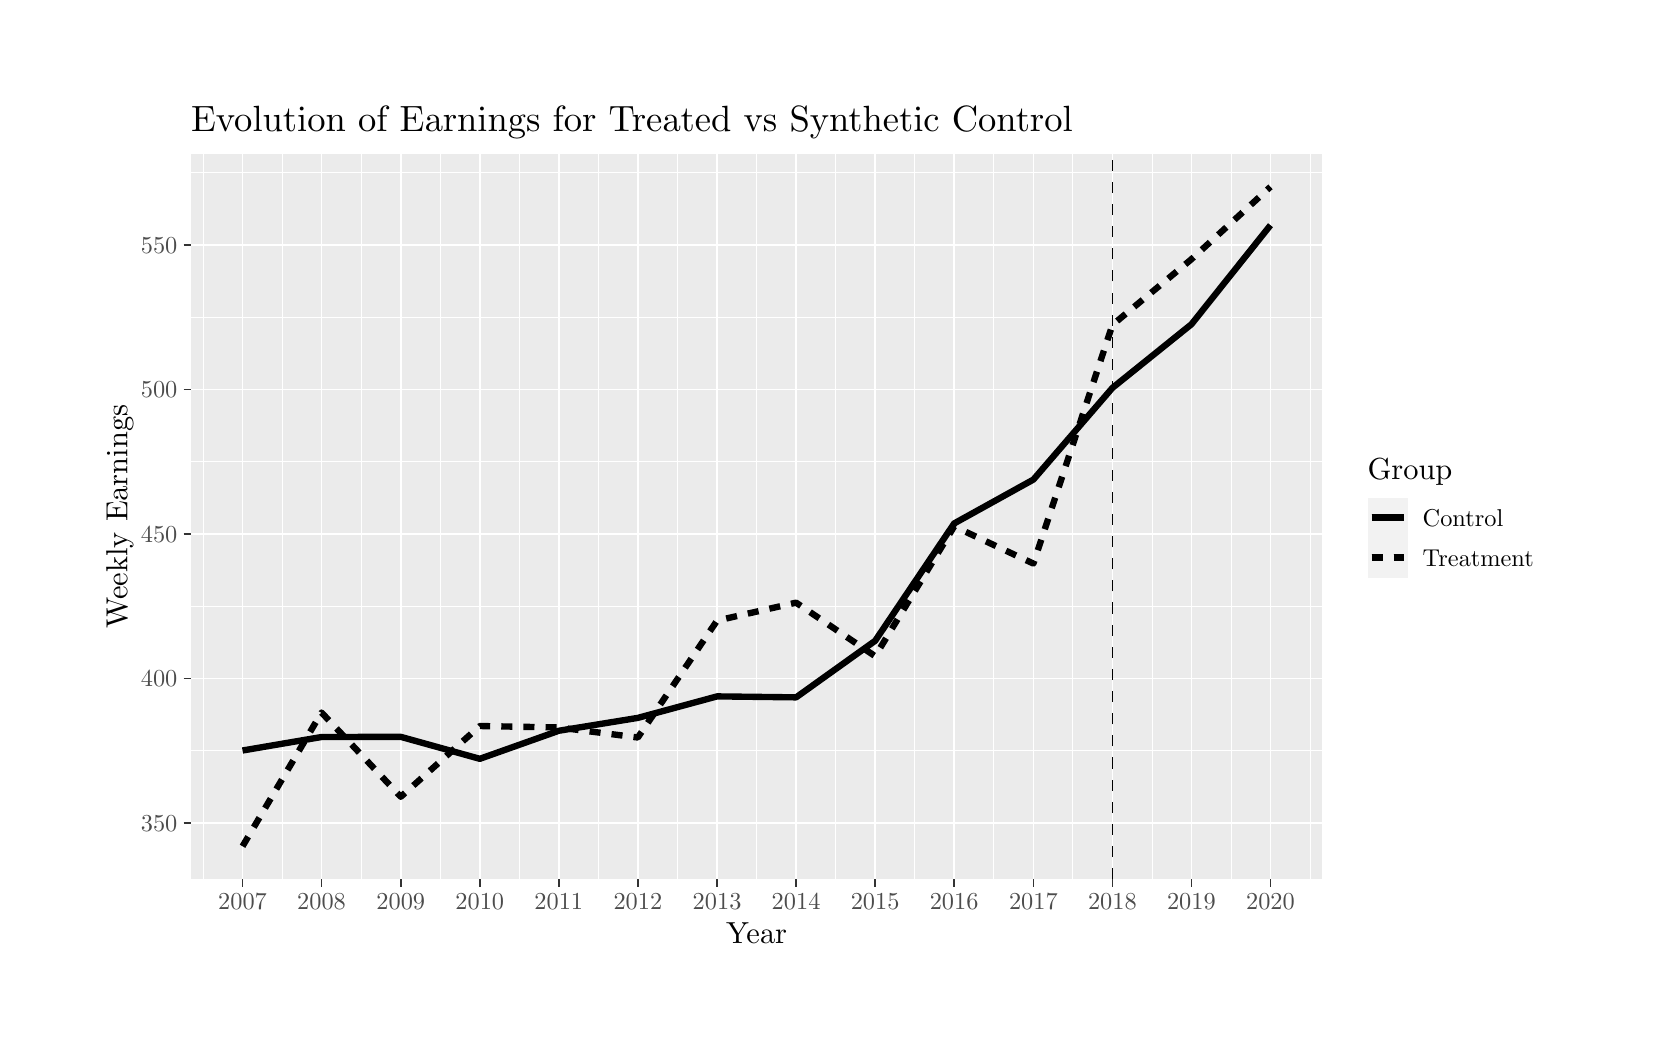
\begin{tikzpicture}[x=1pt,y=1pt]
\definecolor{fillColor}{RGB}{255,255,255}
\path[use as bounding box,fill=fillColor,fill opacity=0.00] (0,0) rectangle (578.16,361.35);
\begin{scope}
\path[clip] (  0.00,  0.00) rectangle (578.16,361.35);
\definecolor{drawColor}{RGB}{255,255,255}
\definecolor{fillColor}{RGB}{255,255,255}

\path[draw=drawColor,line width= 0.6pt,line join=round,line cap=round,fill=fillColor] (  0.00,  0.00) rectangle (578.16,361.35);
\end{scope}
\begin{scope}
\path[clip] ( 59.06, 53.64) rectangle (467.65,315.74);
\definecolor{fillColor}{gray}{0.92}

\path[fill=fillColor] ( 59.06, 53.64) rectangle (467.65,315.74);
\definecolor{drawColor}{RGB}{255,255,255}

\path[draw=drawColor,line width= 0.3pt,line join=round] ( 59.06,100.06) --
	(467.65,100.06);

\path[draw=drawColor,line width= 0.3pt,line join=round] ( 59.06,152.29) --
	(467.65,152.29);

\path[draw=drawColor,line width= 0.3pt,line join=round] ( 59.06,204.53) --
	(467.65,204.53);

\path[draw=drawColor,line width= 0.3pt,line join=round] ( 59.06,256.76) --
	(467.65,256.76);

\path[draw=drawColor,line width= 0.3pt,line join=round] ( 59.06,309.00) --
	(467.65,309.00);

\path[draw=drawColor,line width= 0.3pt,line join=round] ( 63.36, 53.64) --
	( 63.36,315.74);

\path[draw=drawColor,line width= 0.3pt,line join=round] ( 91.91, 53.64) --
	( 91.91,315.74);

\path[draw=drawColor,line width= 0.3pt,line join=round] (120.51, 53.64) --
	(120.51,315.74);

\path[draw=drawColor,line width= 0.3pt,line join=round] (149.10, 53.64) --
	(149.10,315.74);

\path[draw=drawColor,line width= 0.3pt,line join=round] (177.65, 53.64) --
	(177.65,315.74);

\path[draw=drawColor,line width= 0.3pt,line join=round] (206.21, 53.64) --
	(206.21,315.74);

\path[draw=drawColor,line width= 0.3pt,line join=round] (234.80, 53.64) --
	(234.80,315.74);

\path[draw=drawColor,line width= 0.3pt,line join=round] (263.40, 53.64) --
	(263.40,315.74);

\path[draw=drawColor,line width= 0.3pt,line join=round] (291.95, 53.64) --
	(291.95,315.74);

\path[draw=drawColor,line width= 0.3pt,line join=round] (320.50, 53.64) --
	(320.50,315.74);

\path[draw=drawColor,line width= 0.3pt,line join=round] (349.10, 53.64) --
	(349.10,315.74);

\path[draw=drawColor,line width= 0.3pt,line join=round] (377.69, 53.64) --
	(377.69,315.74);

\path[draw=drawColor,line width= 0.3pt,line join=round] (406.25, 53.64) --
	(406.25,315.74);

\path[draw=drawColor,line width= 0.3pt,line join=round] (434.80, 53.64) --
	(434.80,315.74);

\path[draw=drawColor,line width= 0.3pt,line join=round] (463.35, 53.64) --
	(463.35,315.74);

\path[draw=drawColor,line width= 0.6pt,line join=round] ( 59.06, 73.94) --
	(467.65, 73.94);

\path[draw=drawColor,line width= 0.6pt,line join=round] ( 59.06,126.18) --
	(467.65,126.18);

\path[draw=drawColor,line width= 0.6pt,line join=round] ( 59.06,178.41) --
	(467.65,178.41);

\path[draw=drawColor,line width= 0.6pt,line join=round] ( 59.06,230.65) --
	(467.65,230.65);

\path[draw=drawColor,line width= 0.6pt,line join=round] ( 59.06,282.88) --
	(467.65,282.88);

\path[draw=drawColor,line width= 0.6pt,line join=round] ( 77.64, 53.64) --
	( 77.64,315.74);

\path[draw=drawColor,line width= 0.6pt,line join=round] (106.19, 53.64) --
	(106.19,315.74);

\path[draw=drawColor,line width= 0.6pt,line join=round] (134.82, 53.64) --
	(134.82,315.74);

\path[draw=drawColor,line width= 0.6pt,line join=round] (163.38, 53.64) --
	(163.38,315.74);

\path[draw=drawColor,line width= 0.6pt,line join=round] (191.93, 53.64) --
	(191.93,315.74);

\path[draw=drawColor,line width= 0.6pt,line join=round] (220.49, 53.64) --
	(220.49,315.74);

\path[draw=drawColor,line width= 0.6pt,line join=round] (249.12, 53.64) --
	(249.12,315.74);

\path[draw=drawColor,line width= 0.6pt,line join=round] (277.67, 53.64) --
	(277.67,315.74);

\path[draw=drawColor,line width= 0.6pt,line join=round] (306.23, 53.64) --
	(306.23,315.74);

\path[draw=drawColor,line width= 0.6pt,line join=round] (334.78, 53.64) --
	(334.78,315.74);

\path[draw=drawColor,line width= 0.6pt,line join=round] (363.41, 53.64) --
	(363.41,315.74);

\path[draw=drawColor,line width= 0.6pt,line join=round] (391.97, 53.64) --
	(391.97,315.74);

\path[draw=drawColor,line width= 0.6pt,line join=round] (420.52, 53.64) --
	(420.52,315.74);

\path[draw=drawColor,line width= 0.6pt,line join=round] (449.08, 53.64) --
	(449.08,315.74);
\definecolor{drawColor}{RGB}{0,0,0}

\path[draw=drawColor,line width= 2.3pt,dash pattern=on 4pt off 4pt ,line join=round] ( 77.64, 65.55) --
	(106.19,113.87) --
	(134.82, 83.43) --
	(163.38,109.00) --
	(191.93,108.48) --
	(220.49,104.85) --
	(249.12,147.10) --
	(277.67,153.58) --
	(306.23,134.23) --
	(334.78,181.13) --
	(363.41,167.70) --
	(391.97,253.93) --
	(420.52,277.68) --
	(449.08,303.83);

\path[draw=drawColor,line width= 2.3pt,line join=round] ( 77.64,100.15) --
	(106.19,105.03) --
	(134.82,105.09) --
	(163.38, 97.15) --
	(191.93,107.29) --
	(220.49,111.94) --
	(249.12,119.71) --
	(277.67,119.36) --
	(306.23,139.79) --
	(334.78,182.20) --
	(363.41,198.05) --
	(391.97,231.19) --
	(420.52,254.17) --
	(449.08,289.97);

\path[draw=drawColor,line width= 0.6pt,dash pattern=on 4pt off 4pt ,line join=round] (391.97, 53.64) -- (391.97,315.74);
\end{scope}
\begin{scope}
\path[clip] (  0.00,  0.00) rectangle (578.16,361.35);
\definecolor{drawColor}{gray}{0.30}

\node[text=drawColor,anchor=base east,inner sep=0pt, outer sep=0pt, scale=  0.88] at ( 54.11, 70.91) {350};

\node[text=drawColor,anchor=base east,inner sep=0pt, outer sep=0pt, scale=  0.88] at ( 54.11,123.15) {400};

\node[text=drawColor,anchor=base east,inner sep=0pt, outer sep=0pt, scale=  0.88] at ( 54.11,175.38) {450};

\node[text=drawColor,anchor=base east,inner sep=0pt, outer sep=0pt, scale=  0.88] at ( 54.11,227.61) {500};

\node[text=drawColor,anchor=base east,inner sep=0pt, outer sep=0pt, scale=  0.88] at ( 54.11,279.85) {550};
\end{scope}
\begin{scope}
\path[clip] (  0.00,  0.00) rectangle (578.16,361.35);
\definecolor{drawColor}{gray}{0.20}

\path[draw=drawColor,line width= 0.6pt,line join=round] ( 56.31, 73.94) --
	( 59.06, 73.94);

\path[draw=drawColor,line width= 0.6pt,line join=round] ( 56.31,126.18) --
	( 59.06,126.18);

\path[draw=drawColor,line width= 0.6pt,line join=round] ( 56.31,178.41) --
	( 59.06,178.41);

\path[draw=drawColor,line width= 0.6pt,line join=round] ( 56.31,230.65) --
	( 59.06,230.65);

\path[draw=drawColor,line width= 0.6pt,line join=round] ( 56.31,282.88) --
	( 59.06,282.88);
\end{scope}
\begin{scope}
\path[clip] (  0.00,  0.00) rectangle (578.16,361.35);
\definecolor{drawColor}{gray}{0.20}

\path[draw=drawColor,line width= 0.6pt,line join=round] ( 77.64, 50.89) --
	( 77.64, 53.64);

\path[draw=drawColor,line width= 0.6pt,line join=round] (106.19, 50.89) --
	(106.19, 53.64);

\path[draw=drawColor,line width= 0.6pt,line join=round] (134.82, 50.89) --
	(134.82, 53.64);

\path[draw=drawColor,line width= 0.6pt,line join=round] (163.38, 50.89) --
	(163.38, 53.64);

\path[draw=drawColor,line width= 0.6pt,line join=round] (191.93, 50.89) --
	(191.93, 53.64);

\path[draw=drawColor,line width= 0.6pt,line join=round] (220.49, 50.89) --
	(220.49, 53.64);

\path[draw=drawColor,line width= 0.6pt,line join=round] (249.12, 50.89) --
	(249.12, 53.64);

\path[draw=drawColor,line width= 0.6pt,line join=round] (277.67, 50.89) --
	(277.67, 53.64);

\path[draw=drawColor,line width= 0.6pt,line join=round] (306.23, 50.89) --
	(306.23, 53.64);

\path[draw=drawColor,line width= 0.6pt,line join=round] (334.78, 50.89) --
	(334.78, 53.64);

\path[draw=drawColor,line width= 0.6pt,line join=round] (363.41, 50.89) --
	(363.41, 53.64);

\path[draw=drawColor,line width= 0.6pt,line join=round] (391.97, 50.89) --
	(391.97, 53.64);

\path[draw=drawColor,line width= 0.6pt,line join=round] (420.52, 50.89) --
	(420.52, 53.64);

\path[draw=drawColor,line width= 0.6pt,line join=round] (449.08, 50.89) --
	(449.08, 53.64);
\end{scope}
\begin{scope}
\path[clip] (  0.00,  0.00) rectangle (578.16,361.35);
\definecolor{drawColor}{gray}{0.30}

\node[text=drawColor,anchor=base,inner sep=0pt, outer sep=0pt, scale=  0.88] at ( 77.64, 42.63) {2007};

\node[text=drawColor,anchor=base,inner sep=0pt, outer sep=0pt, scale=  0.88] at (106.19, 42.63) {2008};

\node[text=drawColor,anchor=base,inner sep=0pt, outer sep=0pt, scale=  0.88] at (134.82, 42.63) {2009};

\node[text=drawColor,anchor=base,inner sep=0pt, outer sep=0pt, scale=  0.88] at (163.38, 42.63) {2010};

\node[text=drawColor,anchor=base,inner sep=0pt, outer sep=0pt, scale=  0.88] at (191.93, 42.63) {2011};

\node[text=drawColor,anchor=base,inner sep=0pt, outer sep=0pt, scale=  0.88] at (220.49, 42.63) {2012};

\node[text=drawColor,anchor=base,inner sep=0pt, outer sep=0pt, scale=  0.88] at (249.12, 42.63) {2013};

\node[text=drawColor,anchor=base,inner sep=0pt, outer sep=0pt, scale=  0.88] at (277.67, 42.63) {2014};

\node[text=drawColor,anchor=base,inner sep=0pt, outer sep=0pt, scale=  0.88] at (306.23, 42.63) {2015};

\node[text=drawColor,anchor=base,inner sep=0pt, outer sep=0pt, scale=  0.88] at (334.78, 42.63) {2016};

\node[text=drawColor,anchor=base,inner sep=0pt, outer sep=0pt, scale=  0.88] at (363.41, 42.63) {2017};

\node[text=drawColor,anchor=base,inner sep=0pt, outer sep=0pt, scale=  0.88] at (391.97, 42.63) {2018};

\node[text=drawColor,anchor=base,inner sep=0pt, outer sep=0pt, scale=  0.88] at (420.52, 42.63) {2019};

\node[text=drawColor,anchor=base,inner sep=0pt, outer sep=0pt, scale=  0.88] at (449.08, 42.63) {2020};
\end{scope}
\begin{scope}
\path[clip] (  0.00,  0.00) rectangle (578.16,361.35);
\definecolor{drawColor}{RGB}{0,0,0}

\node[text=drawColor,anchor=base,inner sep=0pt, outer sep=0pt, scale=  1.10] at (263.36, 30.59) {Year};
\end{scope}
\begin{scope}
\path[clip] (  0.00,  0.00) rectangle (578.16,361.35);
\definecolor{drawColor}{RGB}{0,0,0}

\node[text=drawColor,rotate= 90.00,anchor=base,inner sep=0pt, outer sep=0pt, scale=  1.10] at ( 36.03,184.69) {Weekly Earnings};
\end{scope}
\begin{scope}
\path[clip] (  0.00,  0.00) rectangle (578.16,361.35);
\definecolor{fillColor}{RGB}{255,255,255}

\path[fill=fillColor] (478.65,157.13) rectangle (549.71,212.25);
\end{scope}
\begin{scope}
\path[clip] (  0.00,  0.00) rectangle (578.16,361.35);
\definecolor{drawColor}{RGB}{0,0,0}

\node[text=drawColor,anchor=base west,inner sep=0pt, outer sep=0pt, scale=  1.10] at (484.15,198.11) {Group};
\end{scope}
\begin{scope}
\path[clip] (  0.00,  0.00) rectangle (578.16,361.35);
\definecolor{fillColor}{gray}{0.95}

\path[fill=fillColor] (484.15,177.08) rectangle (498.60,191.54);
\end{scope}
\begin{scope}
\path[clip] (  0.00,  0.00) rectangle (578.16,361.35);
\definecolor{drawColor}{RGB}{0,0,0}

\path[draw=drawColor,line width= 2.3pt,line join=round] (485.59,184.31) -- (497.16,184.31);
\end{scope}
\begin{scope}
\path[clip] (  0.00,  0.00) rectangle (578.16,361.35);
\definecolor{drawColor}{RGB}{0,0,0}

\path[draw=drawColor,line width= 2.3pt,line join=round] (485.59,184.31) -- (497.16,184.31);
\end{scope}
\begin{scope}
\path[clip] (  0.00,  0.00) rectangle (578.16,361.35);
\definecolor{fillColor}{gray}{0.95}

\path[fill=fillColor] (484.15,162.63) rectangle (498.60,177.08);
\end{scope}
\begin{scope}
\path[clip] (  0.00,  0.00) rectangle (578.16,361.35);
\definecolor{drawColor}{RGB}{0,0,0}

\path[draw=drawColor,line width= 2.3pt,dash pattern=on 4pt off 4pt ,line join=round] (485.59,169.86) -- (497.16,169.86);
\end{scope}
\begin{scope}
\path[clip] (  0.00,  0.00) rectangle (578.16,361.35);
\definecolor{drawColor}{RGB}{0,0,0}

\path[draw=drawColor,line width= 2.3pt,dash pattern=on 4pt off 4pt ,line join=round] (485.59,169.86) -- (497.16,169.86);
\end{scope}
\begin{scope}
\path[clip] (  0.00,  0.00) rectangle (578.16,361.35);
\definecolor{drawColor}{RGB}{0,0,0}

\node[text=drawColor,anchor=base west,inner sep=0pt, outer sep=0pt, scale=  0.88] at (504.10,181.28) {Control};
\end{scope}
\begin{scope}
\path[clip] (  0.00,  0.00) rectangle (578.16,361.35);
\definecolor{drawColor}{RGB}{0,0,0}

\node[text=drawColor,anchor=base west,inner sep=0pt, outer sep=0pt, scale=  0.88] at (504.10,166.82) {Treatment};
\end{scope}
\begin{scope}
\path[clip] (  0.00,  0.00) rectangle (578.16,361.35);
\definecolor{drawColor}{RGB}{0,0,0}

\node[text=drawColor,anchor=base west,inner sep=0pt, outer sep=0pt, scale=  1.32] at ( 59.06,323.81) {Evolution of Earnings for Treated vs Synthetic Control};
\end{scope}
\end{tikzpicture}
